\documentclass[11pt]{article}
%Gummi|061|=)
\usepackage{hyperref}
\usepackage[spanish]{babel}
\usepackage[utf8]{inputenc}
\usepackage{pdfpages}
\title{\textbf{Diseño de Software: Klondike}}
\author{Sergio Arroutbi Braojos}
\selectlanguage{spanish}
\date{\today}
%\addtolength{\topmargin}{-0.5in}
\usepackage[bottom=14em]{geometry}
\usepackage{amsmath}
\usepackage{mathtools}

\begin{document}

\hypersetup
{   
pdfborder={0 0 0}
}
   
\maketitle

\pagebreak

\tableofcontents

\pagebreak

\section{Introducción}
En este ejercicio se ha realizado el análisis, diseño y posterior implementación del juego del klondike. Este juego de cartas, también conocido como ``solitario'', es un juego en el que un único jugador interviene en el reparto y operación de las cartas. El tablero de cartas está formado por la baraja inicial, conocida como ``Deck'', el ``Waste'', donde se levantan las cartas de la baraja, una serie de ``Tableaus'', que permiten sacar de forma provisional las cartas del ``Waste'' ordenándolas por número descendente y alternando los colores de las cartas, y finalmente las ``Foundations'', que son cada uno de los palos del ``Deck'' en orden ascendente.

En cada turno, el jugador puede sacar cartas del ``Deck'' al ``Waste'', colocar cartas del ``Waste'' a los ``Tableaus'' o a las ``Foundations'' y sacar igualmente carta de las ``Foundations'' para seguir combinando cartas en los ``Tableaus''.
El motivo de este documento no es describir de forma muy detallada el juego, que puede consultarse en el siguiente enlace: \url{https://en.wikipedia.org/wiki/Klondike_(solitaire)}
Además, existen ciertas reglas que son configurables en el juego, como el número de cartas del ``Deck'' que se ocultan en cada ronda de la baraja al ``Waste'', el número de veces que el ``Waste'' se puede dar la vuelta hacia el ``Deck''.

Para realizar la implementación software de este juego de cartas se han realizado las diversas fases involucradas en el proceso de desarrollo unificado con diseño orientado a objetos. En este proceso se ha llevado a cabo la idea ``BDUF'' (Big Design Up Front), para el cual se han seguido las siguientes fases:

\begin{itemize}\itemsep0pt
\item{Captura de Requisitos}
\item{Análisis}
\item{Diseño}
\item{Implementación}
\item{Pruebas}
\end{itemize}

En los siguientes capítulos se describen cada una de las anteriores fases y la aproximación que se ha llevado a cabo con el objetivo de llegar a una implementación con un objetivo final: \textbf{Llegar a un software con un buen diseño orientado a objetos}, cuya mantenibilidad sea lo más sencilla posible, y caracterizado por las cuatro premisas que este tipo de diseño trata de alcanzar:

\begin{itemize}\itemsep0pt
\item{Abstracción}
\item{Encapsulación}
\item{Modularidad}
\item{Jerarquía}
\end{itemize}

Para ello, se ha procurado implentar una jerarquía de clases de la mayor calidad posible, caracterizadas por ser :
\begin{itemize}\itemsep0pt
\item{de Bajo Acoplamiento}. Es decir, tener poca relación de fuerza entre unas claes y otras.
\item{Cohesivas}. Por cohesión, nos referimos a la fuerza de ligadura entre los miembros de una clase.
\item{Suficientes}. Por suficiencia se entiende que la clase proporciona suficientes características para proporcionar lo que la abstracción supone cuando interactúe con ellas.
\item{Completas}. Las clases deben ser completas, de forma que capture todas las características que la abstracción supone de ellas.
\item{Primitivas}. De forma que las clases pueden ser implementadas de forma efectiva simplemente proporcionando acceso a las capas inferiores.
\end{itemize}

Con las anteriores características en mente se describe cada una de las distintas fases desarrolladas hasta la implementación final.

\pagebreak

\section{Captura de Requisitos}

Para la captura de requisitos no se ha seguido ninguna metodología especial. El hecho de que el juego Klondike esté ya documentado e implementado permite dar una idea del funcionamiento del mismo.

Por esto, la principal fuente de requisitos para el desarrollo del juego han sido, en este caso, la documentación existente:
Por otro lado, a modo de ``Hands-On'', se ha utilizado el juego ``aisleriot'', implementación del klondike en la distribución Ubuntu de Linux.
A parte de lo descrito anteriormente, se han presentado ciertas características adicionales que pueden suponer ``motivos de cambio'' a considerar en el diseño de la aplicación, como son:

\begin{enumerate}\itemsep0pt
\item{El juego debería estar basado en opciones de menú a través de texto}. Sin embargo, no debería resultar muy difícil el portado del juego para que tuviera interfaz gráfico.
\item{Se podrá cambiar de tipo de baraja (baraja de póquer/baraja española)}. En el caso en el que se utilice la baraja española, la aceptación de cartas en los ``Tableaus'' será por ``palo distinto'', en lugar de ``color distinto'', como ocurre con la baraja francesa.
\item{El diseño debería facilitar el poder cambiar el tipo de reparto de cartas en el Deal de forma sencilla}.
\item{El diseño debería facilitar que el número de Tableaus se pudiera modificar de forma sencilla}.
\end{enumerate}

\pagebreak

\section{Fase de Análisis}
La fase de análisis es, simplemente, un \textbf{``diseño preliminar''}. Se considera que esta fase de análisis se debe de llevar a cabo en una quinta parte del tiempo toal respecto a la fase de diseño.

En esta fase de análisis, en el cual la solución al proceso de desarrollo empieza a tomar forma, se debe dar una primera visión interna del sistema, de forma que empiezan a aflorar los primeros diagramas estructurados por clases estereotipadas, y suele recoger aquellos detalles del dominio propios de los objetos tangibles del desarrollo en cuestión.

En esta fase se debe empezar a comprender la forma del sistema por parte de los desarrolladores. En el caso del klondike, el análisis da lugar a un diagrama estructurado como el que sigue: 

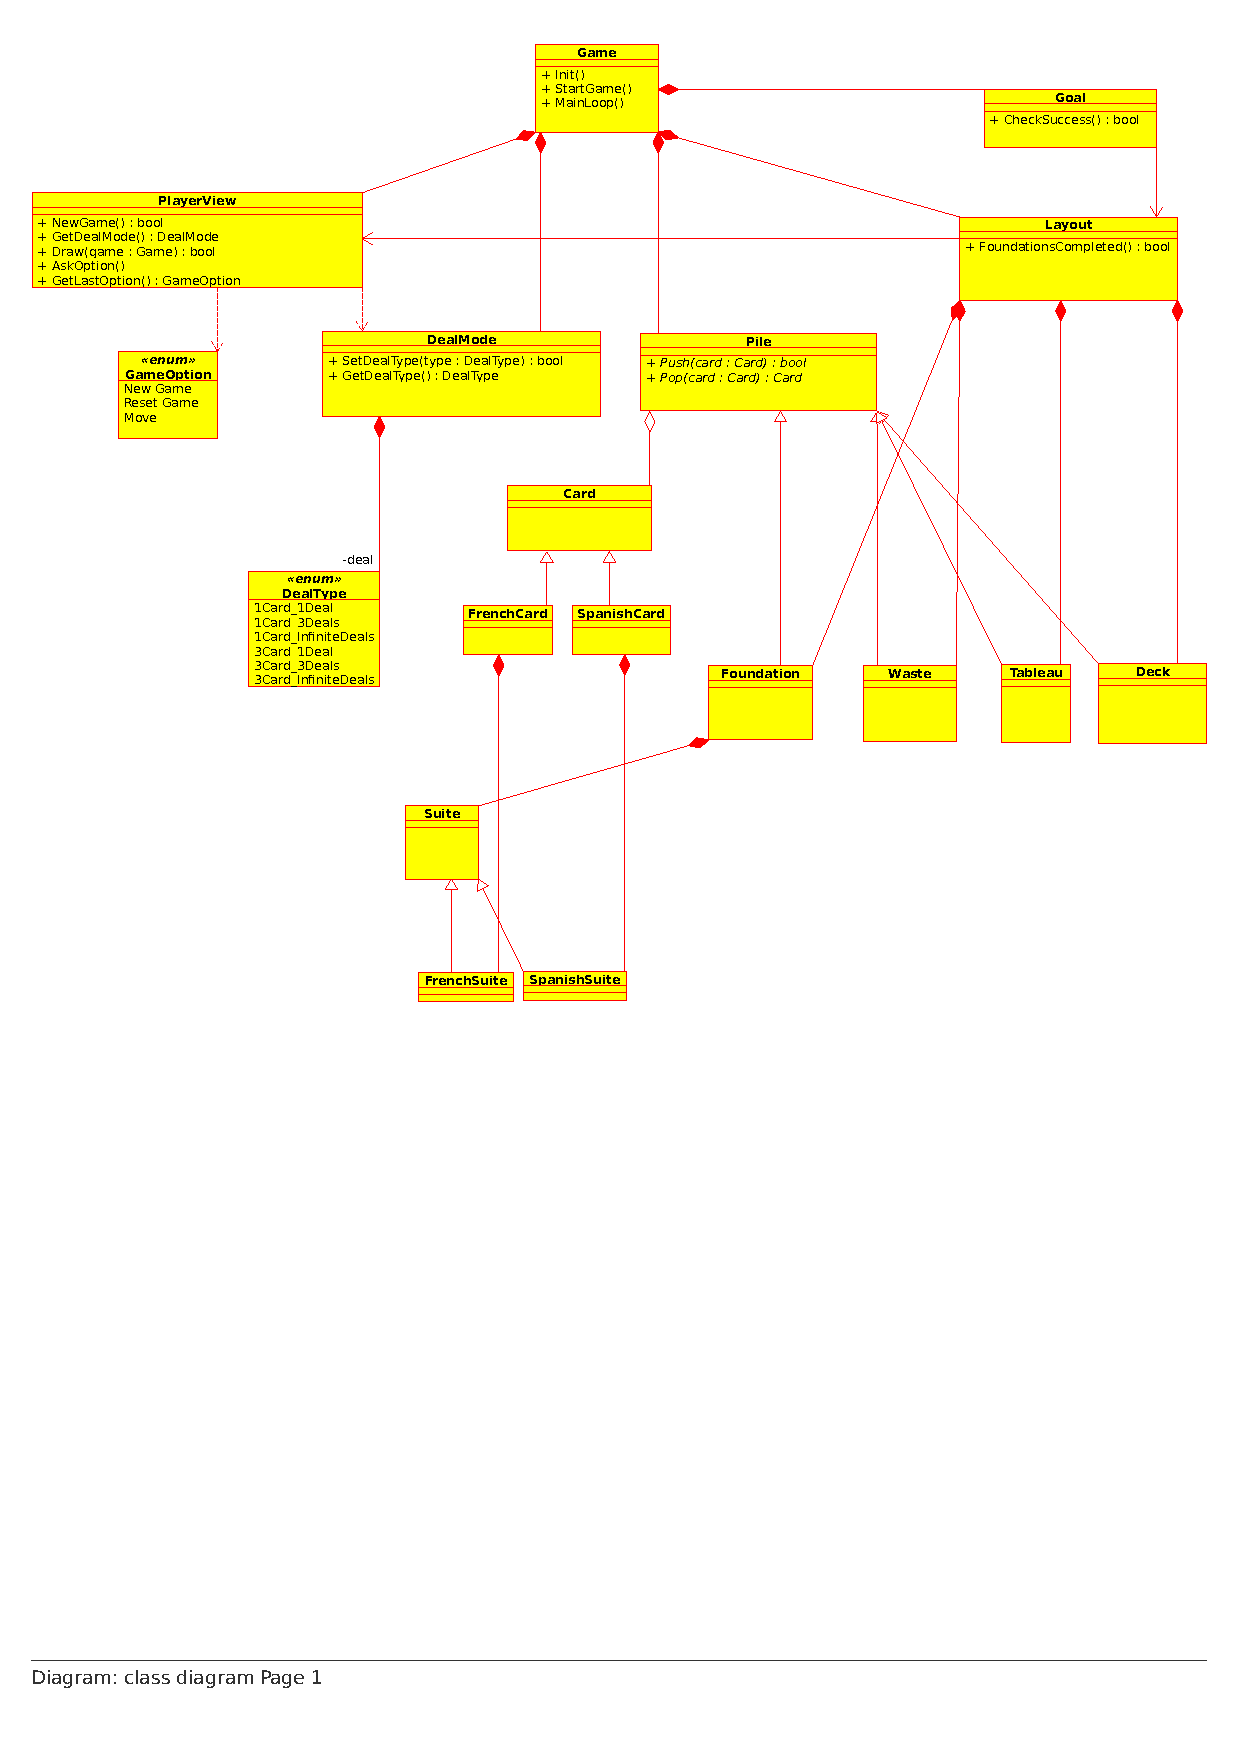
\includepdf[pages=-]{analysis00.pdf}

En este análisis preliminar se muestra un primer boceto de la jerarquía de clases. Para ello, se han identificado los distintos tipos de clases que formarán la jerarquía de clases que permitan implementar el juego.

A continuación se describe de forma resumida cada una de ellas:

\section{Fase de Diseño}
\subsection{Fase de Diseño}

\section{Fase de Implementación}

\end{document}
